
        \subsubsection{Product Perspective}

            The Melanoma Detect App (MDApp) will provide the user with a risk assessment of a skin lesion. The App will guide the user through the process of capturing an image and confirming the correct recognition of the boundary of the lesion. Once confirmed the App will analyse the visual features of the lesion based on dermatological rules and provide the user with an initial risk assessment.

    The App should help motivate the user to make an appointment with a dermatologist when a significant risk has been detected. It is not meant to replace the need to visit a dermatologist though.

    In order to provide these services the MDApp must be able to utilise the features and capabilities of the smart phone that it runs on. The Partial Context Diagram in figure ~\ref{fig:partial_feature_tree} shows the MDApp in relation to the external components that it must interface with. Email, camera, and file system are system components within the smart phone that the app must communicate with. The border extraction and risk assessment services are online services that the MDApp must send image data to in order to receive the border data and risk assessment. Finally, to make it all work together, the MDApp must provide an interface to the user that is clear and unobtrusive, guiding the user through all the necessary steps.


            \begin{figure}[H]
                \centering
                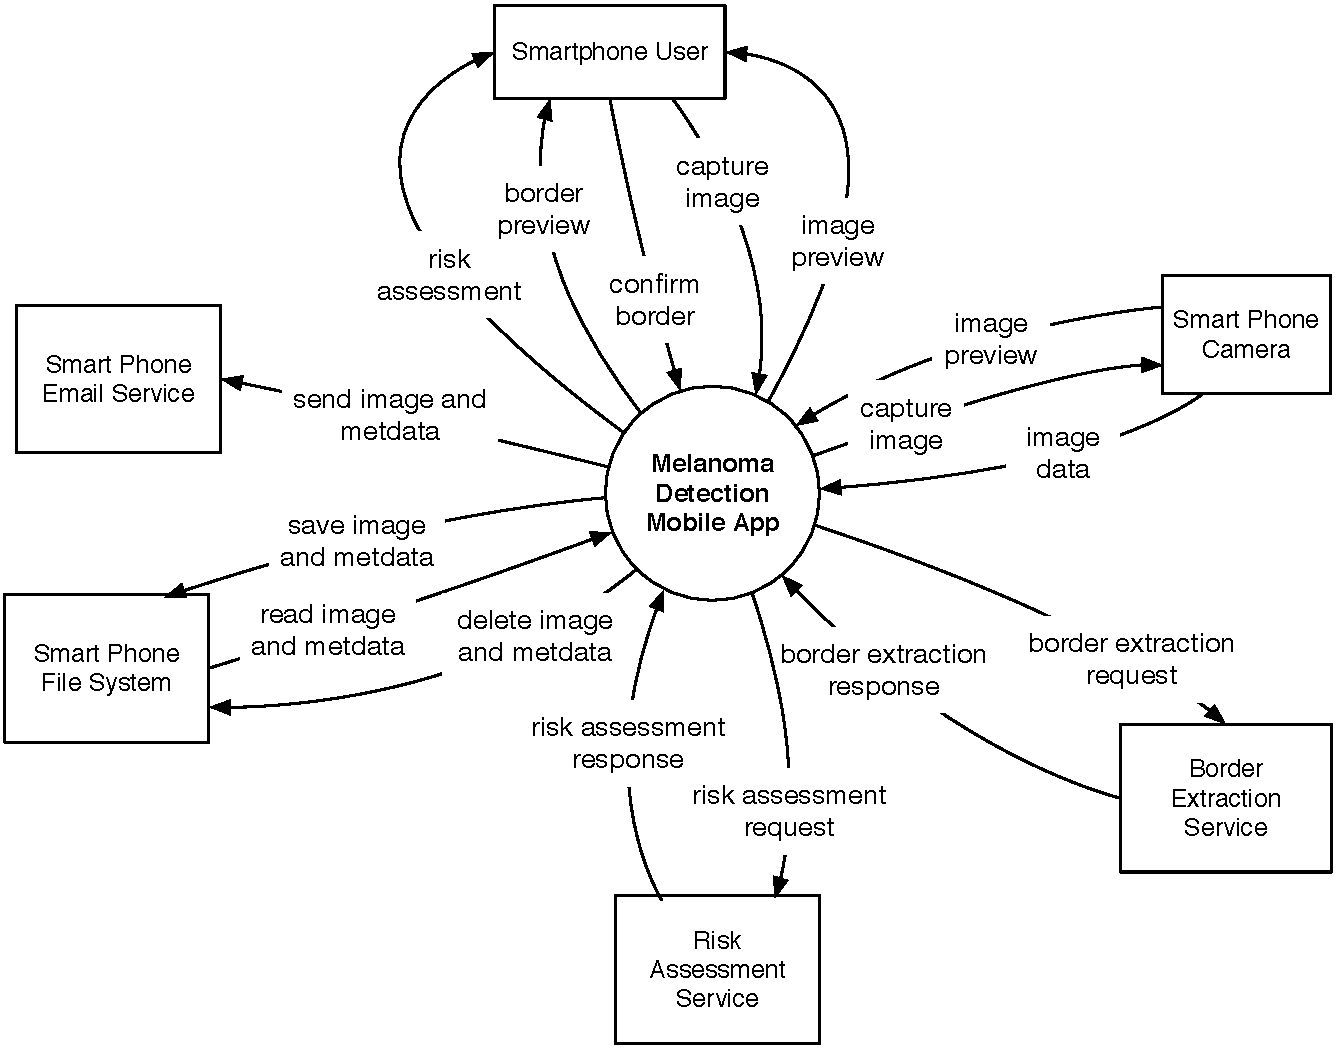
\includegraphics[width=\textwidth]{assets/requirements/ContextDiagram.pdf}
                \caption{Context Diagram of the Melanoma Detection App}
                \label{fig:partial_feature_tree}
            \end{figure}


        \subsubsection{User Classes and Characteristics}

            The Melanoma Detection App only has one class of user, the Smartphone User. The Smartphone User has one or several skin lesions that she or he is worried about.
The Smartphone User is not expected to have any technical or dermatological expertise.

        \subsubsection{Operating Environment}

                    \noindent
                    \begin{itemize}[leftmargin=*]
                        \item[]  \textbf{OE-1} : The Mobile App shall operate on the following platforms: Android OS (minumum v.5.2.2) and iOS (minumum v.9.3)

                    \end{itemize}


        \subsubsection{Design and Implementation Constraints}

                    \noindent
                    \begin{itemize}[leftmargin=*]
                        \item[]  \textbf{CO-1} : The Border Extraction and Risk Assessment Services shall be implemented on a server in oder to leverage the effort already made with python and python based libraries for image processing and scientific calculations. Wifi access is therefore a requirement for the app to run.
                        \item[]  \textbf{CO-2} : The method for archiving images and risk assessment data will use whatever standard is the most accepted for the relevant platform. i.e. iCloud on iOS.


                    \end{itemize}

        \subsubsection{Assumptions and Dependencies}

                    \noindent
                    \begin{itemize}[leftmargin=*]
                        \item[]  \textbf{AS-1} : It is assumed that the user of the software is also the user of the mobile phone. The software might need to request permission from the user to access the camera or network.

                    \end{itemize}

                    \noindent
                    \begin{itemize}[leftmargin=*]
                        \item[]  \textbf{AS-2} : It is assumed that the user of the software is also the only user of the mobile phone. Therefore no additional measures need be taken to secure the app from other potiential users of the phone. The app will be as secure as the phone itself.

                    \end{itemize}